\documentclass[letterpaper,11pt]{article}
\usepackage{graphicx}
\usepackage{listings}
\usepackage[super]{nth}
\usepackage[hyphens]{url}
\usepackage{hyperref}
\usepackage{amsmath}
\usepackage[makeroom]{cancel}
\usepackage[table]{xcolor}
\usepackage{comment}
\usepackage[space]{grffile}

\newcommand*{\srcPath}{../src}%

\lstset{
	basicstyle=\footnotesize,
	breaklines=true,
}

\begin{document}

\begin{titlepage}

\begin{center}

\Huge{Assignment 3}

\Large{CS 532:  Introduction to Web Science}

\Large{Spring 2017}

\Large{Grant Atkins}

\Large Finished on \today

\end{center}

\end{titlepage}

\newpage


% =================================
% First question
% =================================
\section*{1}


\subsection*{Question}

\begin{verbatim}
1.  Write a Python program that extracts 1000 unique links from
Twitter.  You might want to take a look at:

http://adilmoujahid.com/posts/2014/07/twitter-analytics/

see also:

http://docs.tweepy.org/en/v3.5.0/index.html
https://github.com/bear/python-twitter
https://dev.twitter.com/rest/public

But there are many other similar resources available on the web.
Note that only Twitter API 1.1 is currently available; version 1
code will no longer work.

Also note that you need to verify that the final target URI (i.e.,
the one that responds with a 200) is unique.  You could have many
different shortened URIs for www.cnn.com (t.co, bit.ly, goo.gl,
etc.).  For example:

$ curl -IL --silent https://t.co/DpO767Md1v | egrep -i "(HTTP/1.1|^location:)"
HTTP/1.1 301 Moved Permanently
location: https://goo.gl/40yQo2
HTTP/1.1 301 Moved Permanently
Location: https://soundcloud.com/roanoketimes
/ep-95-talking-hokies-recruiting-one-week-before-signing-day
HTTP/1.1 200 OK

You might want to use the search feature to find URIs, or you can
pull them from the feed of someone famous (e.g., Tim O'Reilly).  If
you find something inappropriate for any reason you see fit, just
discard it and get some more links.  We just want 1000 links that
were shared via Twitter.

Hold on to this collection and upload it to github -- we'll use it
later throughout the semester.
\end{verbatim}

\subsection*{Answer}

To first approach this problem I started out with the the template code provided by Adil Moujahid in a blog post about twitter analytics \cite{twitterstreamref}. I liked the fact that you could get tweets real time so I followed this approach of streaming tweets live, only later did I realize this took approximately 12 hours to get unique URIs. I wrote this code in python 3.6 and used the following dependencies:

\begin{itemize}
  \item requests
  \item tweepy
\end{itemize}

The tweepy library allows the developer to stream tweets based on keywords. For my keywords I chose some of my favorite jazz and funk musicians and bands that were saved to my youtube playlist at the time, \url{https://www.youtube.com/playlist?list=PLYcZodEQpdPcZjZks1IV2V9nMPWNvzoxK}, to filter these streams.

The main program for twitter streaming was \textbf{tweepyCrawler.py} shown in Listing \ref{lst:q1tweepy}. It first starts by listening to the stream of data from twitters streaming API. Then once a a piece of data is received in JSON format, I parsed the number of mementos found in the JSON key ``urls'' which provided the urls of a tweet. The JSON could also have a $``retweeted\char`_status''$ key which would contain more URIs provided from the tweet referenced, so I also included those URIs.

\lstinputlisting[frame=single,caption={Python script for twitter streaming},label=lst:q1tweepy,captionpos=b,numbers=left,showspaces=false,showstringspaces=false,basicstyle=\footnotesize]{\srcPath/tweepyCrawler.py}

Since I was taking live tweets it was inevitable that I would get repeating URIs, inappropriate URIs, or just javascript based HTML pages with no content. Therefore, when receiving the JSON I would perform an HTTP get request to the URI provided with the User-Agent ``Mozilla/5.0.'' Then I would check if the final URI was already in my output file, if it wasn't I would add it. I also added a blacklist of URIs and domain types that were in the bad category. Sometimes this searching for unique URIs didn't work, especially when it came to youtube URIs that had extra parameters inside them. To compensate for this I created \textbf{filterUnwanted.py} shown Listing \ref{lst:q1filter} in and \textbf{removeDuplicates.py} shown in Listing \ref{lst:q1duplicates}. The first script would strip youtube of their extra parameters except for their video ids and it would also remove bad URIs. The second script would make sure all the URIs were still unique in the file, removing duplicates if they were found. Finally I saved all of these URIs to a text file, \textbf{finalURIs.txt} \cite{finalurisref}.

\lstinputlisting[frame=single,caption={Python script for filtering and cleaning data files},label=lst:q1filter,captionpos=b,numbers=left,showspaces=false,showstringspaces=false,basicstyle=\footnotesize]{\srcPath/filterUnwanted.py}

\lstinputlisting[frame=single,caption={Python script for removing duplicates in data files},label=lst:q1duplicates,captionpos=b,numbers=left,showspaces=false,showstringspaces=false,basicstyle=\footnotesize]{\srcPath/filterUnwanted.py}


\clearpage

% =================================
% Second question
% =================================

\section*{2}

\subsection*{Question}

\begin{verbatim}
2.  Download the TimeMaps for each of the target URIs.  We'll use the ODU 
Memento Aggregator, so for example:

URI-R = http://www.cs.odu.edu/

URI-T = http://memgator.cs.odu.edu/timemap/link/http://www.cs.odu.edu/

or:

URI-T = http://memgator.cs.odu.edu/timemap/json/http://www.cs.odu.edu/

(depending on which format you'd prefer to parse)

Create a histogram* of URIs vs. number of Mementos (as computed
from the TimeMaps).  For example, 100 URIs with 0 Mementos, 300
URIs with 1 Memento, 400 URIs with 2 Mementos, etc.  The x-axis
will have the number of mementos, and the y-axis will have the
frequency of occurence.

* = https://en.wikipedia.org/wiki/Histogram

What's a TimeMap?  
See: http://www.mementoweb.org/guide/quick-intro/
And the week 4 lecture. 
\end{verbatim}

\clearpage

\subsection*{Answer}

For this problem I used  \url{http://memgator.cs.odu.edu/} and wrote \textbf{timeMap.py} to retrieve a JSON response for the time maps of my 1000 URIs. If the response was ``404 not found'' it was assumed that there were no mementos for the URI. If there was a JSON response, I took the count of all archives provided in the JSON key ``list''. For each response I saved the URI and the count to a CSV file named \textbf{timeMaps.csv}. I then created a simple histogram, using R shown in Listing \ref{lst:q2timemapR}, of URIs vs. Number of Mementos as shown in Figure \ref{fig:q2histogram}. An overwhelming majority of the URIs had either no mementos or a very low amount.

\lstinputlisting[frame=single,caption={R script for creating Histogram},label=lst:q2timemapR,captionpos=b,numbers=left,showspaces=false,showstringspaces=false,basicstyle=\footnotesize]{\srcPath/timeMapMementos.R}

\begin{figure}[h]
\centering
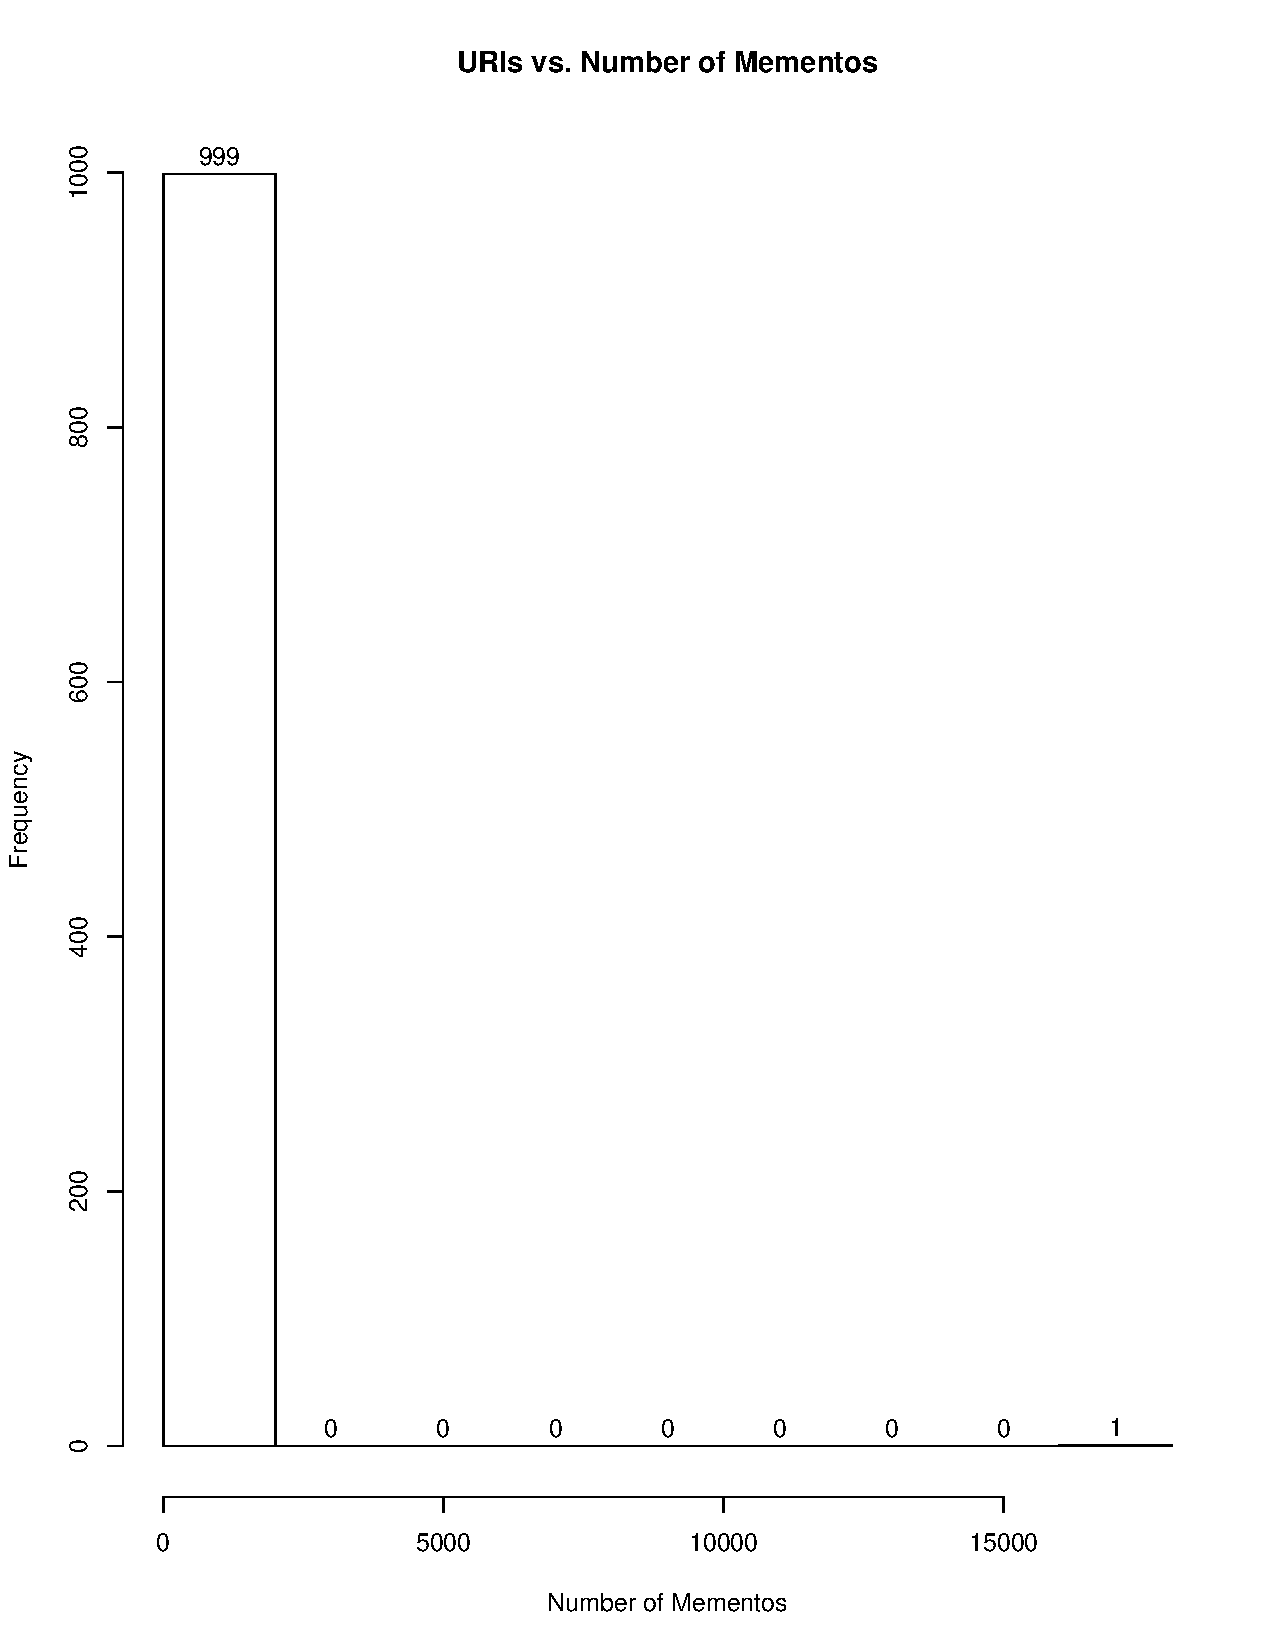
\includegraphics[scale=0.6]{timemapHistogram.pdf}
\caption{Histogram of Number of URIs vs. Number of Mementos}
\label{fig:q2histogram}
\end{figure}


\clearpage

% =================================
% Third question
% =================================

\section*{3}

\subsection*{Question}

\begin{verbatim}
3.  Estimate the age of each of the 1000 URIs using the "Carbon
Date" tool:

http://ws-dl.blogspot.com/2016/09/2016-09-20-carbon-dating-web-version-30.html

Note: you should use "docker" and install it locally.  You can do
it like this:

http://cd.cs.odu.edu/cd?url=http://www.cs.odu.edu/

But it will inevitably crash when everyone tries to use it at the
last minute.

For URIs that have > 0 Mementos and an estimated creation date,
create a graph with age (in days) on the x-axis and number of
mementos on the y-axis.

Not all URIs will have Mementos, and not all URIs will have an
estimated creation date.  Show how many fall into either categories.
For example,

total URIs:         1000
no mementos:     137  
no date estimate:  212
\end{verbatim}

\clearpage
\subsection*{Answer}

Using the memento counts retrieved from question 2, I used the carbon dating tool provided in the question to retrieve the estimated creation dates for each of these URIs \cite{carbondateref}. For each response I saved the URI and the ``Estimated Creation Date'' JSON key to a CSV file named \textbf{carbonDate.csv}. The code used to complete this task is displayed in Listing \ref{lst:q2carbondatepy}. 

\lstinputlisting[frame=single,caption={Python script for retrieving estimated creation date},label=lst:q2carbondatepy,captionpos=b,numbers=left,showspaces=false,showstringspaces=false,basicstyle=\footnotesize]{\srcPath/carbonDate.py}

Once I retrieved all of the dates I merged both the \textbf{carbonDate.csv} and \textbf{timeMaps.csv} together on their URIs using \textbf{mergeCSVs.py}, shown in Listing \ref{lst:q3mergepy}. At the same time if the URI had an estimated creation date, the number of days difference from the current date (02/09/2017) to the date provided would be determined. Finally I created a scatter plot, built using R shown in Listing \ref{lst:q2carbonDateR}, depicting the the Days vs. Number of Mementos shown in Figure \ref{fig:scatterplot}. I later applied a log-log scale to both axes to show the values more distributed, otherwise most of the values would have been lying flat along the x-axis due to low memento counts, this is shown in Figure \ref{fig:scatterplot2}.

The following values were found using \textbf{carbonDateMementos.R}:
\begin{itemize}
  \item total URIs:	     1000
  \item no mementos:      949
  \item no date estimate: 266
\end{itemize}

It was found that URIs that had no date estimates also didn't contain any mementos.

\lstinputlisting[frame=single,caption={Python script to merge CSVs and determine date},label=lst:q3mergepy,captionpos=b,numbers=left,showspaces=false,showstringspaces=false,basicstyle=\footnotesize]{\srcPath/mergeCSVs.py}

\clearpage

\lstinputlisting[frame=single,caption={R Script to find create scatterplot and determine values},label=lst:q2carbonDateR,captionpos=b,numbers=left,showspaces=false,showstringspaces=false,basicstyle=\footnotesize]{\srcPath/carbonDateMementos.R}

\begin{figure}[h]
\centering
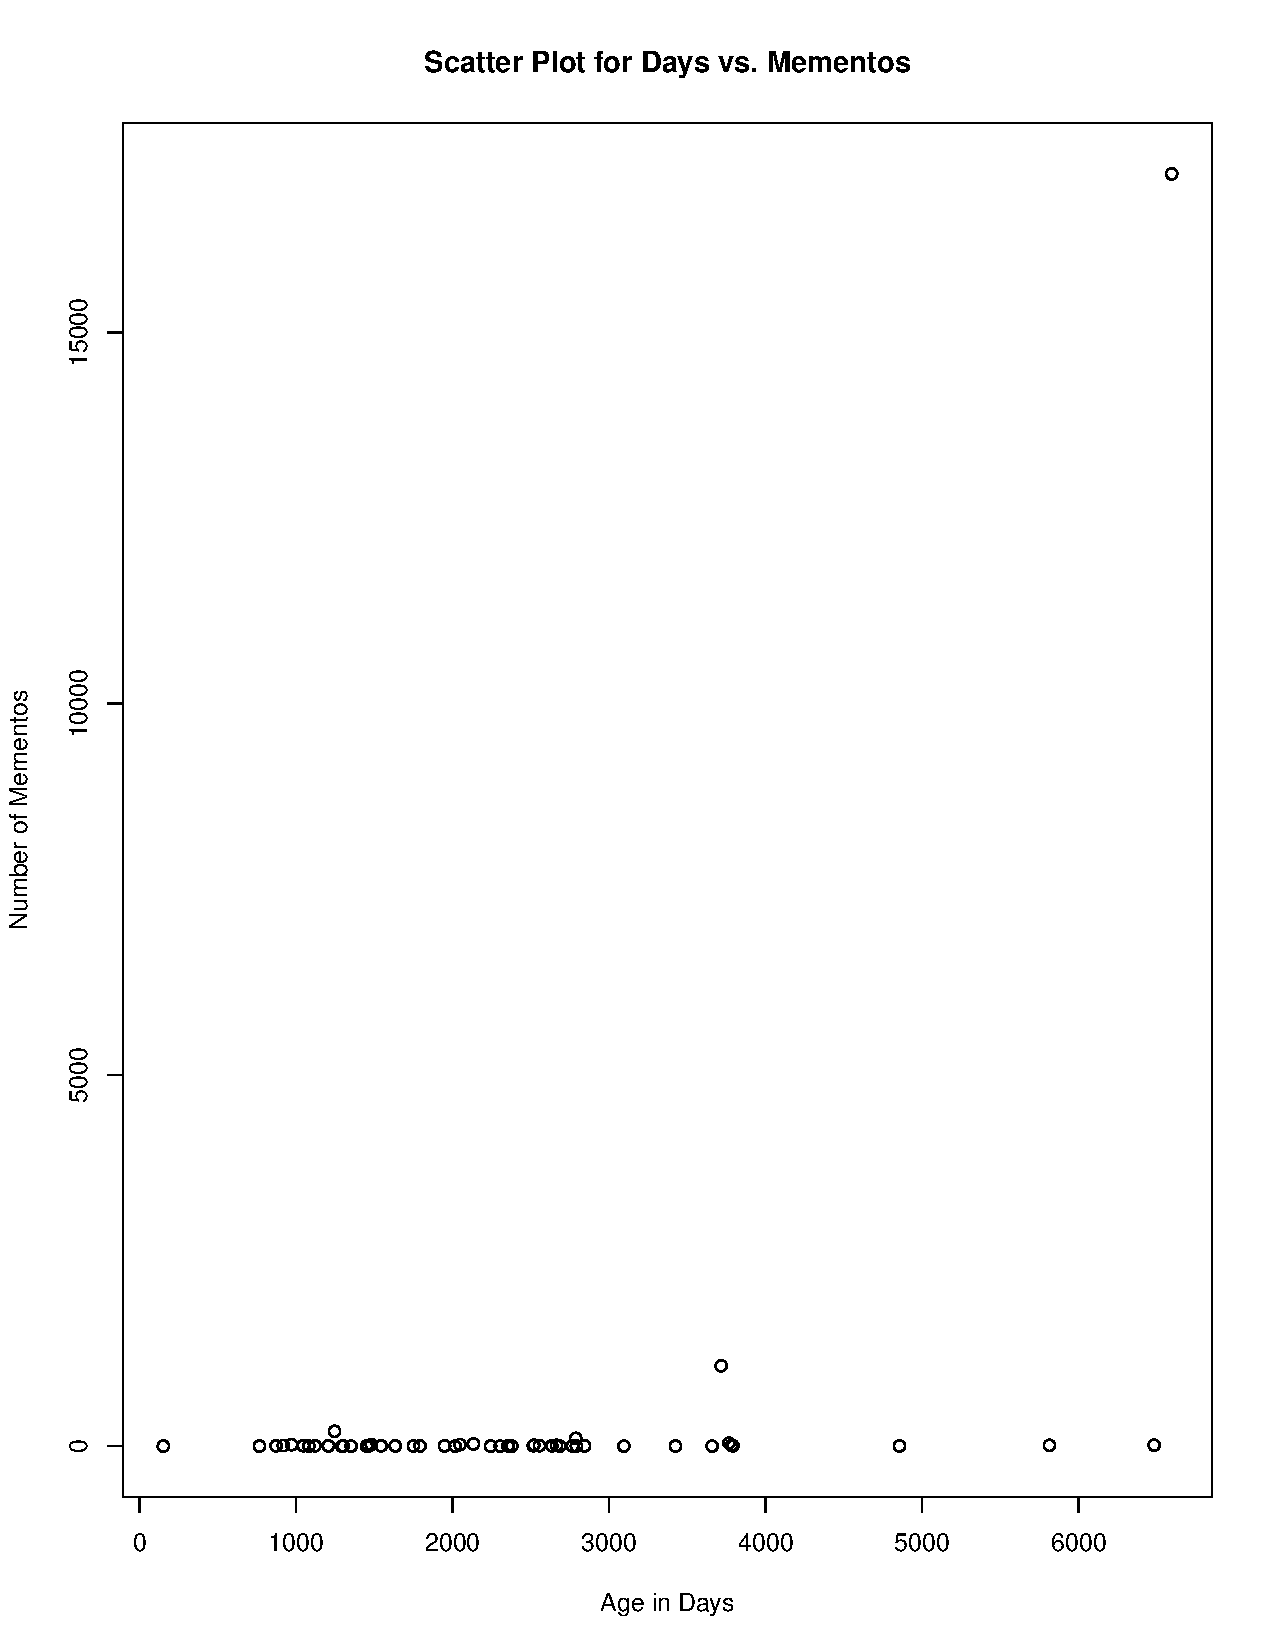
\includegraphics[scale=0.6]{carbonDateScatterplot.pdf}
\caption{Scatter plot of age in days and number of mementos}
\label{fig:scatterplot}
\end{figure}

\clearpage

\begin{figure}[h]
\centering
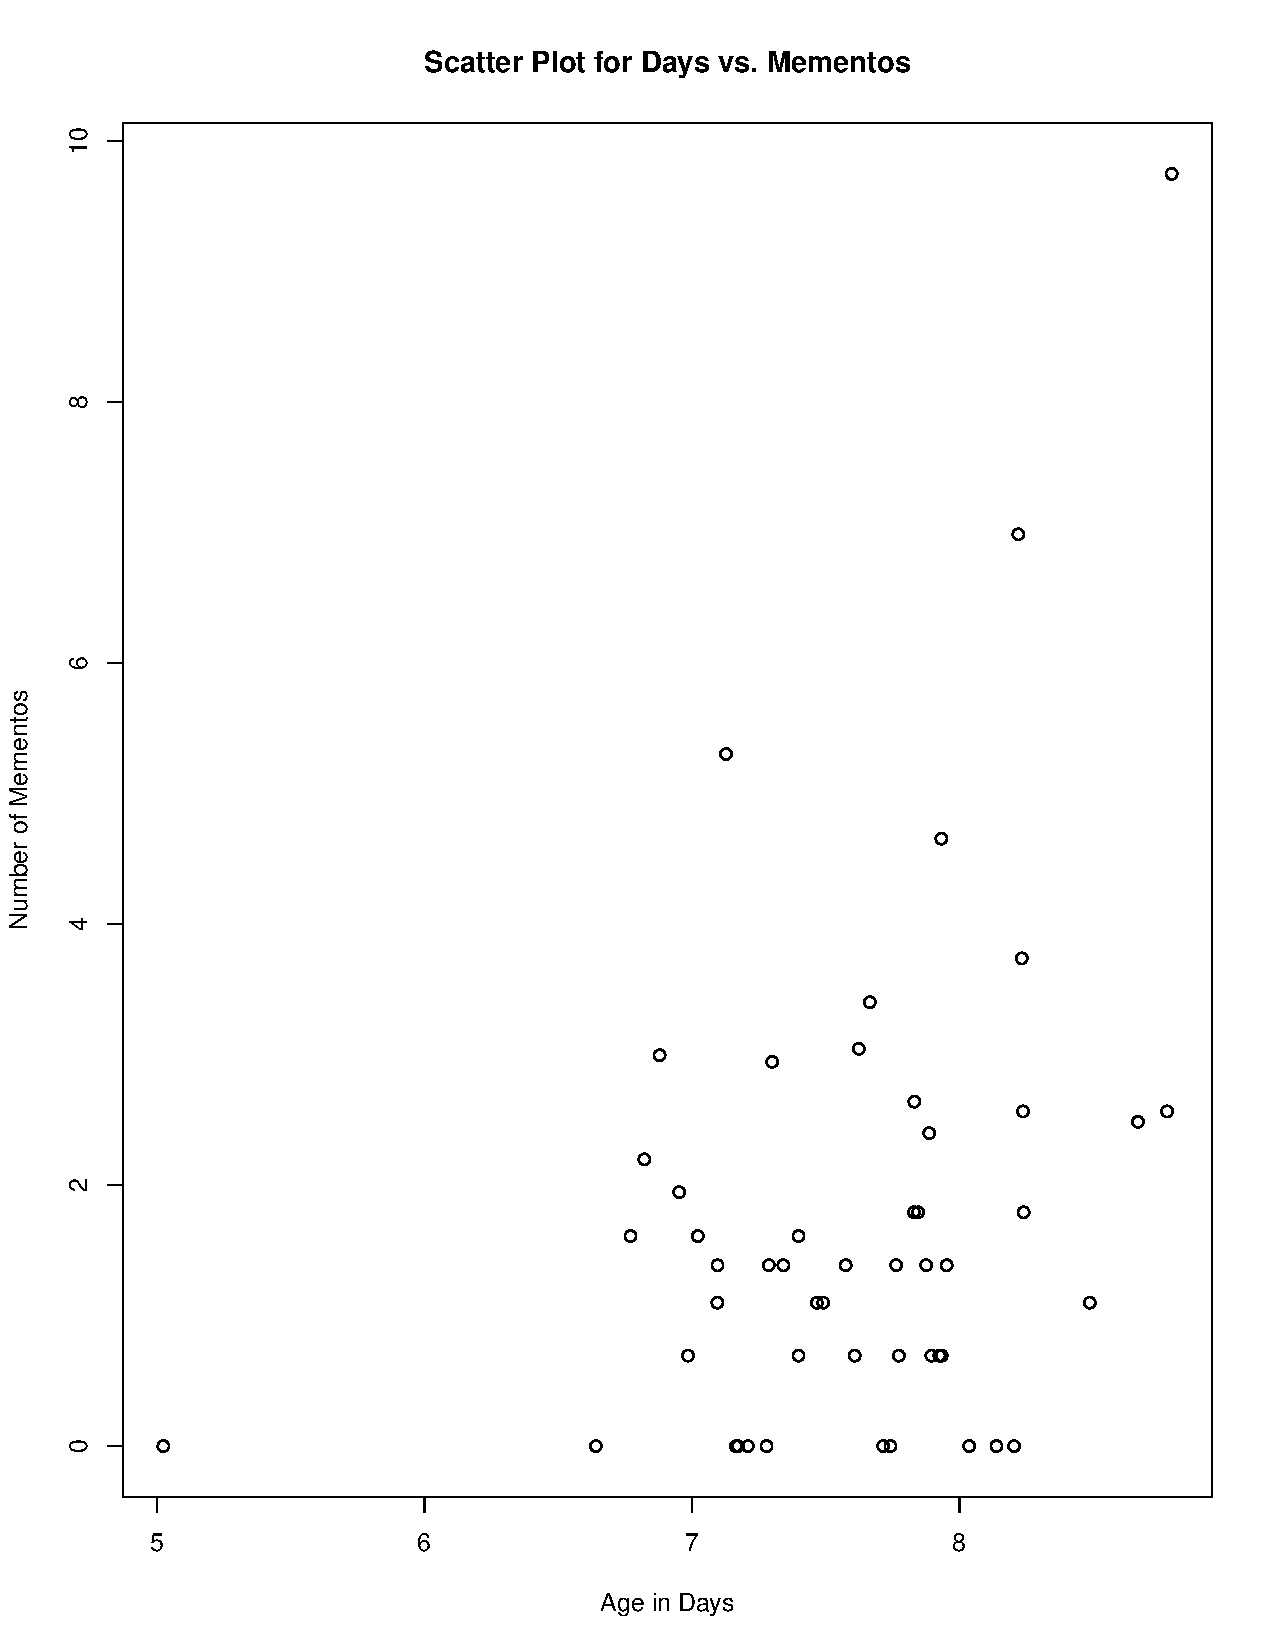
\includegraphics[scale=0.6]{carbonDateScatterplot2.pdf}
\caption{Scatter plot of age in days and number of mementos with log-log scale}
\label{fig:scatterplot2}
\end{figure}

\clearpage

% =================================
% Bibliography
% =================================

\begin{thebibliography}{9}
\bibitem{finalurisref}
Atkins, Grant. ``finalURIs.txt - Twitter scraped URIs.'' cs532-s17 Github Repository. N.p., 09 Feb. 2017. Web. 09 Feb. 2017.\url{https://github.com/grantat/cs532-s17/blob/master/assignments/A2/src/output/finalURIs.txt}
\bibitem{twitterstreamref} 
Moujahid, Adil. ``An Introduction to Text Mining Using Twitter Streaming API and Python.'' An Introduction to Text Mining Using Twitter Streaming API and Python // Adil Moujahid // Data Analytics and More. N.p., 21 July 2014. Web. 08 Feb. 2017. \url{http://adilmoujahid.com/posts/2014/07/twitter-analytics/}
\bibitem{carbondateref}
Zetan, Li. ``2016-09-20: Carbon Dating the Web, Version 3.0.'' 2016-09-20: Carbon Dating the Web, Version 3.0. N.p., 20 Sept. 2016. Web. 08 Feb. 2017. \url{http://ws-dl.blogspot.com/2016/09/2016-09-20-carbon-dating-web-version-30.html}
\end{thebibliography}

\end{document}